\section{KNN Classification} \label{knn}
In this section, we are focusing on using k--nearest neighbors (also known as KNN) algorithm to fit our data. To prepare for our KNN model, we apply one-hot encoding to transform all the categorical features with n possible values into n binary features, in order to make sure our KNN model can measure the ``distance" between categorical features well.

Our first attempt with KNN is trying to fit a model on all the features. Earlier when we finish our data cleaning process, we have 23 features left, however, after we perform one-hot encoding to all categorical features, we now have 101 columns. As KNN is known for computationally expensive, with a large amount of feature, it took 19 hours to test our KNN model with 10 fold cross-validation using 50 different value of $k$'s. Despite the long processing time, we only achieve a accuracy of 70.44\% on the test data. 

Next thing we tried is reducing feature columns in order to reduce running time and to increase model accuracy. By examining the data, we started with deleting columns containing more than 9 levels. Then, we applied \texttt{evimp} function in \texttt{earth} package to help us determine which columns are of more importance to the model. We ended up choosing 22 ``important" columns among the original 101 ones. For a variable, the more model subsets can be generated by \texttt{earth}’s backward pass, the more important the variable is. By doing so, not only we reduce the run time for the model from 19 hours to 30 minutes, we also increase the accuracy to 76.64\%. The confusion matrix is shown below in Figure \ref{fig:knnConf}, and the model accuracy associated with our choice of $k$'s in shown in Figure \ref{fig:knn_k}. For our data set, a small $k=5$ or $7$ seems work the best. 

\begin{figure}[h]
    \centering
    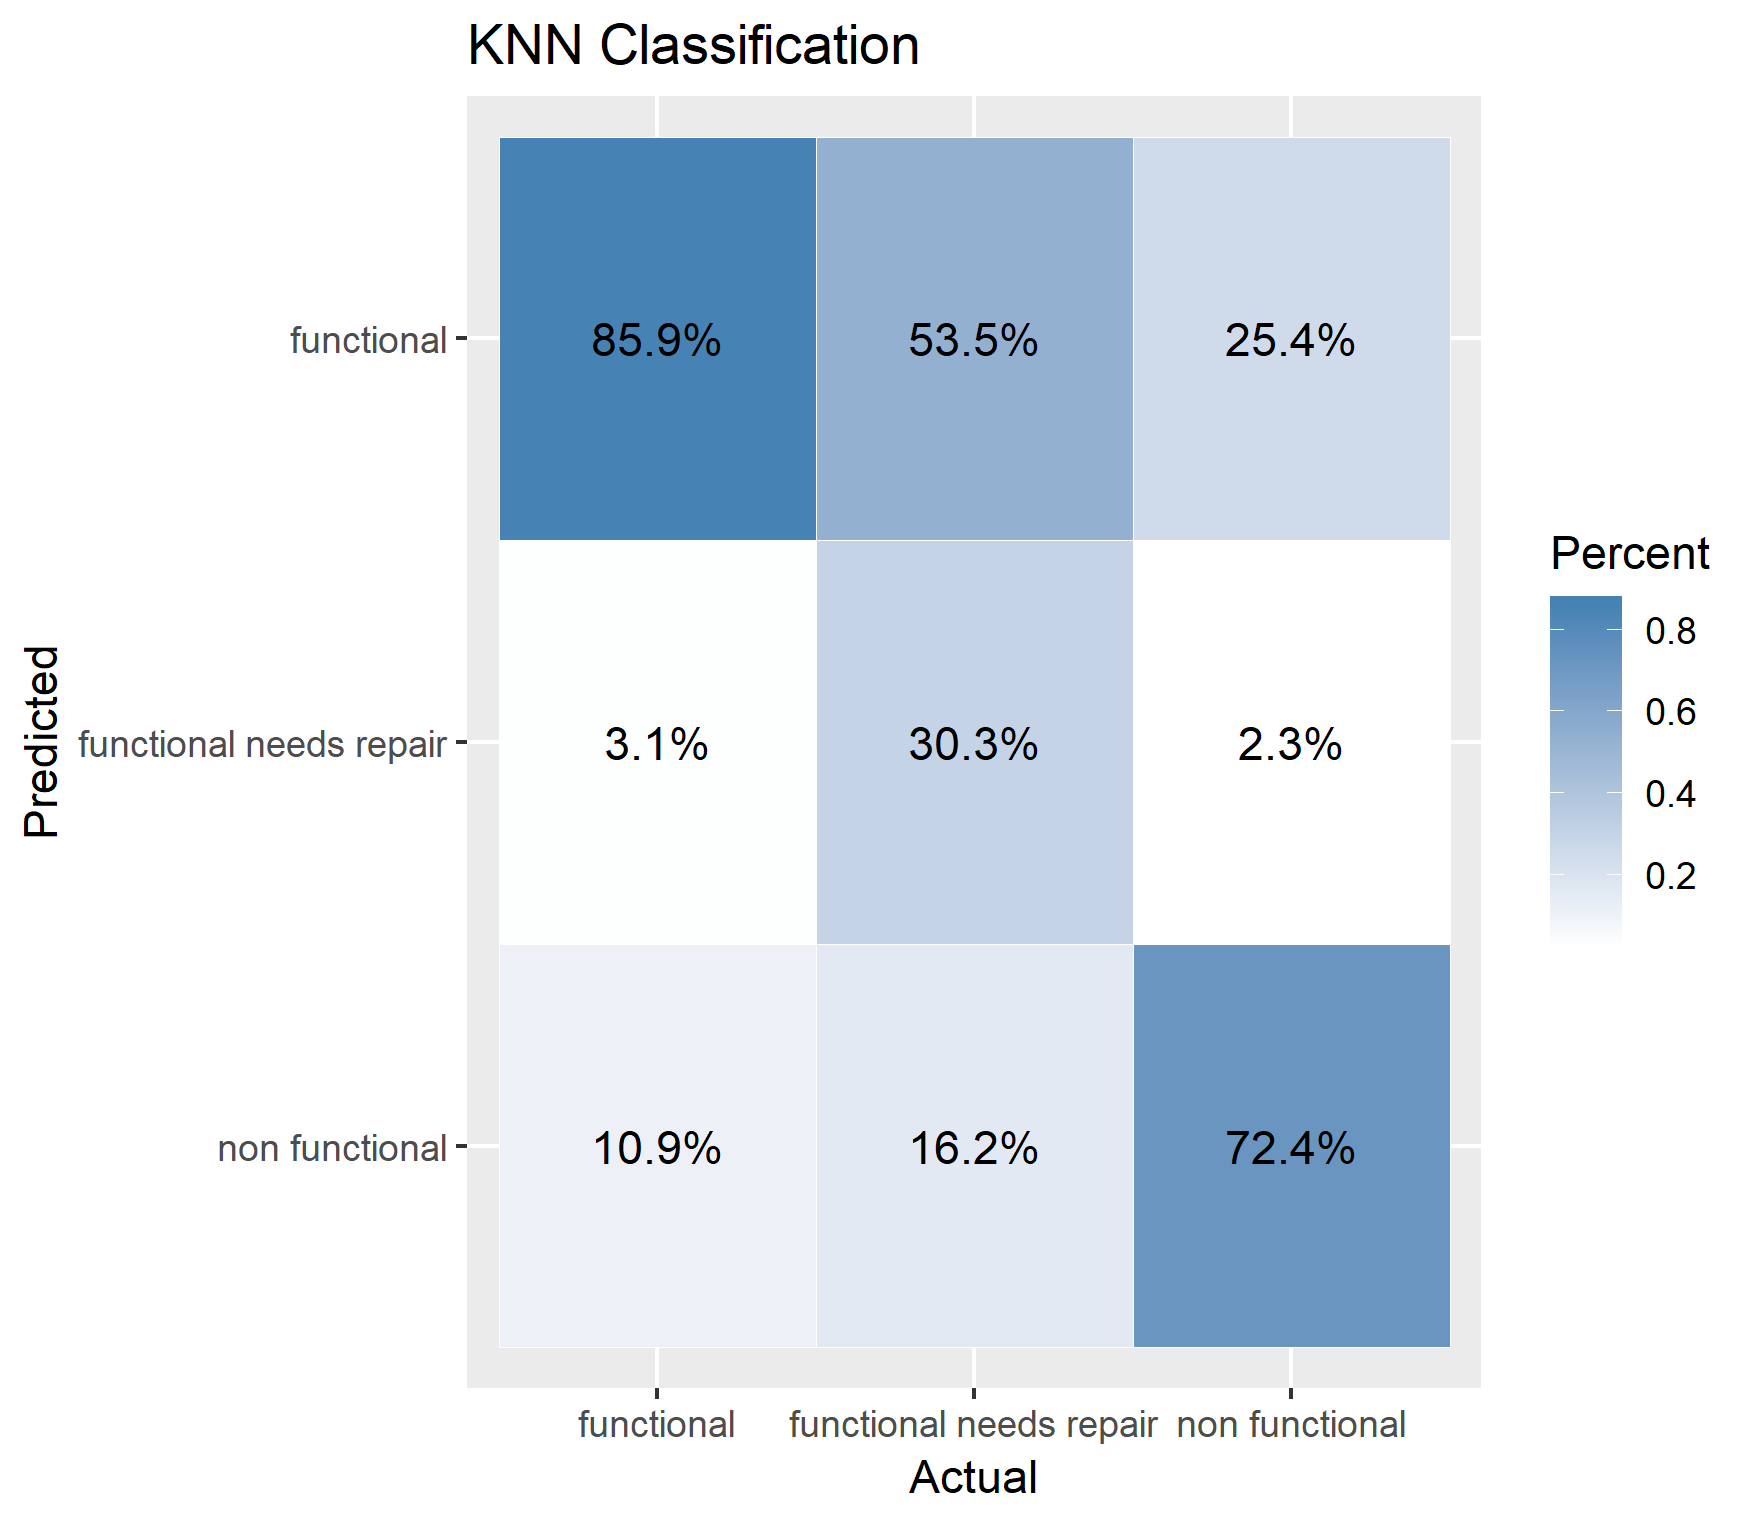
\includegraphics[width = 0.7\textwidth]{Figures/KNNConfMatrix.png}
    \caption{KNN confusion matrix}
    \label{fig:knnConf}
\end{figure}


\begin{figure}[h]
    \centering
    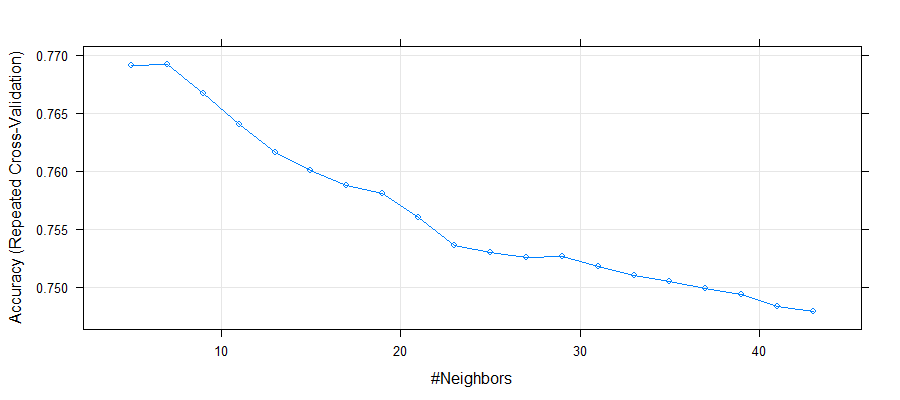
\includegraphics[width = \textwidth]{Figures/knnplot.png}
    \caption{KNN model with different K's}
    \label{fig:knn_k}
\end{figure}

As we observed from above confusion matrix and other models we tried, while the model predicts the ``functional" and ``non functional'' class relatively well, our accuracy on ``functional needs repair'' class are far from satisfying. Taking a look back at our data set, there is only 7\% data are in the ``functional needs repair'' class, and this imbalanced issue leads to low accuracy of this class. We adapt Synthetic Minority Over-sampling Technique(SMOTE) to help us ``create" more minority class samples. The overall accuracy of KNN model after we re-sampling the data using SMOTE decreases to 71.03\%, however, the average accuracy between three classes increases from 62.87\% to 66.82\%, and the accuracy on ``functional needs repair'' class increased from 30.3\% to 68.5\%. Eventually, it's a trade-off between overall and average accuracy. 